\begin{frame}{What is {\it Scheduling}?}
  \vspace{0.3cm}
  \begin{block}{Definition {\small \it \color{blue!50!black!50}[Pinedo, 2008]}}
    Scheduling deals with the allocation of {\bf resources} to {\bf tasks} over
    given \textbf{time} periods and its goal is to optimize one or more \textbf{objectives}.
  \end{block}
\pause
  \vspace{0.3cm}
  {\bf Goal:} Decide when execute the tasks, i.e. when allocate resources
  to the tasks.
\pause
\vspace{0.3cm}

  Sometimes also how much resources give to the tasks.
  \vspace{0.5cm}
 {\small  \begin{description}[constraints :]
    \pause
  \item[tasks :]  courses, landing/taking off, step in project,
    production operation... 
    \pause
  \item[constraints :]
    \begin{itemize}
    \item temporal $\rightarrow$ deadline, precedence, setup...
    \item resource $\rightarrow$ availability, nature... 
    \end{itemize}
    \pause
  \item[objective :] resource consumption, total cost, makespan...
  \end{description}}
\vfill
\end{frame}


\begin{frame}
  \frametitle{The Cumulative Scheduling Problem} 
  \vspace{0.1cm}
  \textbf{Inputs : }
  \vspace{0.15cm}
  \begin{itemize}
  \item a set ${\cal A}=\{1,\dots ,n\}$ of {\bf non-preemptive} tasks
    \vspace{0.15cm}
  \item a {\bf cumulative} and {\bf renewable} resource available in quantity $B$
    \vspace{0.15cm}
  \item for each task:
    \vspace{-1cm}
    \begin{columns}
      \hfill
      \begin{column}{0.36\linewidth}
        \begin{itemize}
        \item \footnotesize  a processing time $p_i$
        \item \footnotesize a resource consumption $b_i$ 
        \item \footnotesize a release date $r_i$ and a deadline $d_i$ 
        \end{itemize}
      \end{column}
      \begin{column}{0.7\linewidth}
        \centering
        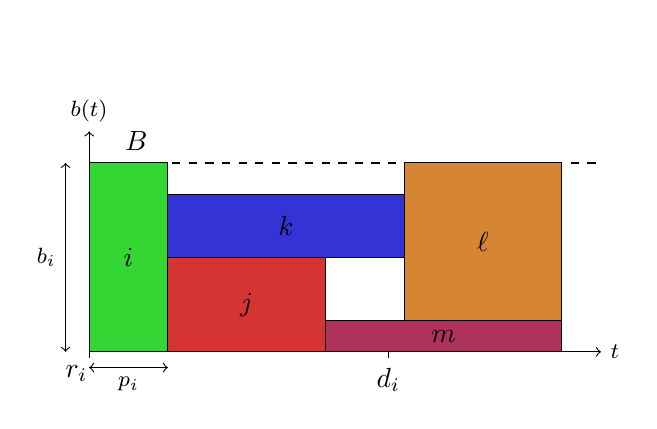
\begin{tikzpicture}
  [yscale=0.4]
  \node at (0,10) {};

  \node[label={[shift={(-0.4,-0.5)}]}] (O) at (0,0) {};
  \draw[fill=red!80!black!80] (1,0) rectangle (3,3)   node[midway] {$j$};
  \draw[dashed,thick] (0,6)   -- (6.5,6);
  \node at (0.6,6.7)  {$B$};
    \draw[<->] (0,-0.5) -- (1,-0.5) node[midway,below] {\footnotesize $p_i$};
    \draw[<->] (-0.3,0) -- (-0.3,6) node[midway,left] {\footnotesize $b_{i}$};
  
  \draw (0,0) -- (0,-0.2) node[below=0.2cm,left=-0.1cm] {$r_i$};
  \draw (3.8,0) -- (3.8,-0.2) node[below] {$d_i$};
  
  \draw[fill=green!80!black!80] (0,0) rectangle (1,6)   node[midway] {$i$};
  \draw[fill=blue!80!black!80] (1,3) rectangle (4,5)   node[midway] {$k$};
  \draw[fill=orange!80!black!80] (4,1) rectangle (6,6)   node[midway] {$\ell$};
  \draw[fill=purple!80!black!80] (3,0) rectangle (6,1)   node[midway] {$m$};
  \draw[->] (O.center) -- (0,7) node[above] {\footnotesize $b(t)$};
  \draw[->] (O.center) -- (6.5,0) node[right] {\footnotesize $t$};


\end{tikzpicture}

      \end{column} 
    \end{columns}
  \end{itemize}
  \vspace{-0.5cm}
  \textbf{Application : }
  \vfill
  \begin{itemize}
  \item electricity consumption cannot exceed a certain level.
  \end{itemize}
\end{frame}

\begin{frame}{Continuous/Discrete resource} 
  \begin{description}
  \item[Continuous resource:] ~
  \end{description}
  
  \vspace{-0.3cm}
  \begin{itemize}
  \item {\small non-integer \textcolor{blue!80!black!80}{allocation}}

    {\footnotesize $\rightarrow$ task $i$ consumes \textcolor{blue!80!black!80}{$\mathbf{3.5}$} units of resource}
  \item {\small non-integer \textcolor{red!80!black!80}{time } }
    
    {\footnotesize $\rightarrow$ task $i$ consumes $3$ units of resource in \textcolor{red!80!black!80}{$\mathbf{[1.5,2]}$}}
  \end{itemize} 

  \vspace{0.2cm} 
  \begin{description}
  \item[  Discrete resource:] ~
  \end{description}

  \vspace{-0.3cm}
  \begin{itemize}
  \item {\small integer \textcolor{blue!80!black!80}{allocation }}

    {\footnotesize $\rightarrow$ task $i$ consumes \textcolor{blue!80!black!80}{$\mathbf{3}$} units of resource}
  \item {\small integer \textcolor{red!80!black!80}{time }}

    {\footnotesize $\rightarrow$ task $i$ consumes $3$ units of resource in \textcolor{red!80!black!80}{$\mathbf{[1,2]}$}}
  \end{itemize}

  \vspace{0.2cm} 
  \begin{center}
    {\footnotesize
      \begin{tabular}{|c|c|c|}
        \hline
        & Continuous Time & Discrete Time\\
        \hline
        Continuous allocation & \cellcolor{blue!80!black!80}&   \cellcolor{blue!50!black!20}\\
        \hline
        Discrete allocation & &  \cellcolor{blue!50!black!20}\\
        \hline
      \end{tabular}}
  \end{center}
\end{frame}


\begin{frame}
  \frametitle{Limitations of the CuSP}
  \vspace{0.5cm}
  \begin{itemize}
  \item {Limitation} : tasks have fixed duration and resource consumption
    \vfill
  \item<2-> But, in practice, it is not always the case\\
  \end{itemize}
  \vspace{0.6cm}
  \begin{columns}
    \hfill
    \begin{column}{0.45\linewidth}
      \centering
      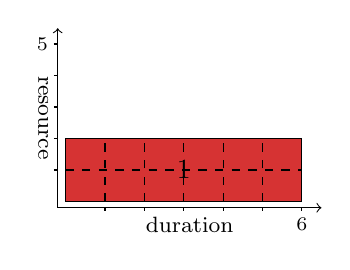
\begin{tikzpicture}
        [xscale=0.5,yscale=0.4]
        \node (O) at (0,0) {};
        \draw[fill=red!80!black!80] (0,0) rectangle (6,2) node[midway] {$1$};
        \draw[->](-0.2,-0.2) -- (-0.2,5.5)
        node[midway,below,rotate=-90] {\footnotesize resource};
        
        
        \draw[->] (-0.2,-0.2) -- (6.5,-0.2) node[midway,below]
        {\footnotesize duration};
        \foreach \i in {1,...,5}{
          \draw (-0.3,\i) -- (-0.2,\i);
          \draw (\i, -0.3) -- (\i,-0.2);
        }
        \onslide<3->{
          \draw (-0.3,5) -- (-0.2,5) node[left] {\scriptsize  $5$};
          \draw (6, -0.3) -- (6,-0.2) node[below] {\scriptsize  $6$};
          \draw[dashed] (0,0) grid (6,2);
        }
      \end{tikzpicture}
    \end{column}
    \hfill
    \begin{column}{0.45\linewidth}
      \centering
      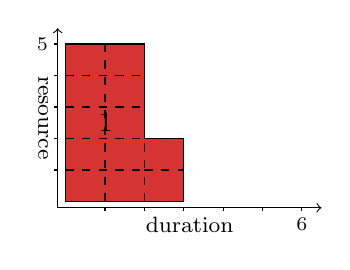
\begin{tikzpicture}
        [xscale=0.5,yscale=0.4]
        \node (O) at (0,0) {};
        \onslide<3->{
          
          \draw[->] (-0.2,-0.2) -- (6.5,-0.2) node[midway,below] {\footnotesize duration};

          \path[draw,fill=red!80!black!80] (0,0) node[above=1cm,right=0.3cm] {$1$}-- (0,5) -- (2,5) -- (2,2) -- (3,2) -- (3,0)-- cycle;
          \draw[->](-0.2,-0.2) -- (-0.2,5.5)
          node[midway,below,rotate=-90] {\footnotesize resource};
          \foreach \i in {1,...,5}{
            \draw (-0.3,\i) -- (-0.2,\i);
            \draw (\i, -0.3) -- (\i,-0.2);}

          \draw (-0.3,5) -- (-0.2,5) node[left] {\scriptsize $5$};
          \draw (6, -0.3) -- (6,-0.2) node[below] {\scriptsize  $6$};
          \draw[dashed] (0,0) grid (2,5);
          \draw[dashed] (2,0) grid (3,2);}
      \end{tikzpicture}
    \end{column}
    \hfill
  \end{columns}

  \vspace{0.3cm}
  \onslide<4->{
    A required {\bf energy} quantity ({\bf [resource $\times$ time]}, e.g. MW/h , pers./day) is associated to a task.
  }
\end{frame}


% \begin{frame}{Motivating Problem
%   {\small \it \color{gray!50!black!50} [Artigues et al., 2013]}} 
%   \vfill
%   \begin{block}{}
%     \begin{center}


%       \vspace{0.2cm}
%       \includegraphics[scale=0.1]{pipe.jpg}

%       \begin{tikzpicture}[yscale=.6]
%         \node (O) at (0,0) {};
%         \draw[-latex,ultra thick, bleuLAAS!100!black!50] (O.center) -- (-3,-1.5);
%         \draw[-latex,ultra thick, bleuLAAS!100!black!50] (O.center) -- (0,-1.5);
%         \draw[-latex,ultra thick, bleuLAAS!100!black!50] (O.center) -- (3,-1.5);

%         \node[draw] at (-3.4,-2.1) {drawing mill}; 
%         \node[draw] at (3.5,-2.1) {pipe-tubing};

%         \node[draw] at (0,-2.1) {\textbf<4>{foundry}};
%       \end{tikzpicture}
%     \end{center}
%   \end{block}
%   \vfill
%   \pause
%   \begin{itemize}
%   \item melting and heating use a {\bf HUGE} quantity of energy
%     \vfill
%     \pause
%   \item $\Rightarrow$ high electricity cost:
%     \begin{itemize}
%     \item total energy consumed
%     \item penalty for power overrun
%     \end{itemize}
%   \end{itemize}
% \end{frame}

\begin{frame}
  \frametitle{Motivating Problem 
    {\small \it \color{gray!50!black!50} [Artigues et al., 2013]}}
  \vfill 
  \begin{block}{\bf \large  pipe-manufacturing plant} 
    melting and heating use a {\bf HUGE} quantity of energy
  \end{block}
  \vfill
  \begin{columns}
    \begin{column}{0.5\linewidth}
      \begin{itemize}
      \item a set of melting jobs
        \vspace{0.4cm}
      \item melting operation has variable duration\\
        {\small (depending of the power given + may vary over time)}
        \vspace{0.4cm}
      \end{itemize}     
    \end{column}
    \hfill 
    \begin{column}{0.4\linewidth}
      \onslide<1->{  \includegraphics[width=0.8\linewidth]{figures/induction.jpg}}
    \end{column}
  \end{columns}
  \vfill
  \begin{itemize}
  \item upper and lower bound on the instantaneous power given \\
    {\small(operational and physical consideration)}
    \vspace{0.4cm}
  \item electrical power limitation\\
    {\small(electrical overrun cost)}
  \end{itemize}
\end{frame}

\begin{frame}
  \frametitle{Literature review}
  \begin{itemize}
    \vfill
  \item {\bf Cumulative Scheduling Problem (CuSP)},
    {\color{gray!50!black!50} \it [Erschler \& Lopez, 1990] }, {\color{blue!80!black!80} fixed resource consumption}
    \vfill
    \pause
  \item {\bf Fully elastic scheduling}, {\color{gray!50!black!50} \it [Baptiste et al., 1999]}, {\color{blue!80!black!80} no upper and lower bound on the consumption}
    \vfill
    \pause
  \item {\bf Variable Intensity}, {\color{gray!50!black!50} \it [Kis, 2005]}, {\color{blue!80!black!80} no lower bound on the consumption}
    \vfill  
    \pause
  \item {\bf Scheduling with continuous resource}, {\color{gray!50!black!50}\it [Blazewicz et al., 2006]}, {\color{blue!80!black!80}  no upper and lower bound}
    \vfill
    \pause
  \item {\bf Multimode activities}, {\color{gray!50!black!50}\it [De Reyck
      et al., 1998]},
    {\color{blue!80!black!80} tasks have rectangular shape}
  \end{itemize}
  \vfill
\end{frame}


\begin{frame}{The CECSP : definition }
  Generalization of the CuSP
  \begin{itemize}
    \vfill
  \item duration $p_i$ $\leftrightarrow$ required energy  $W_i$
    \vfill
  \item fixed resource consumption $b_i$ $\leftrightarrow$ variable
    resource consumption $b_i(t)$ 
    \vfill  
  \item Task can take any shape bounded by:
    \begin{itemize}
    \item its \textcolor<1>{blue!80!black!80!}{time-window}
    \item a \textcolor<1>{green!60!black!80}{maximal and minimal resource consumption}
    \item \textcolor<1>{red!80!black!80}{energy amount} that has to be received by the task
    \end{itemize}
    \vfill
  \end{itemize}
  \begin{overlayarea}{\textwidth}{3cm}
    \only<1> {
      \vfill
      \begin{columns}
        \begin{column}{0.45\linewidth}
          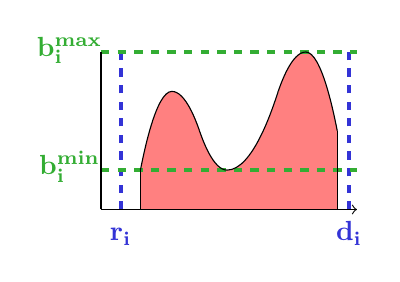
\begin{tikzpicture}
  [scale=0.5]
  \node (O) at (0,0) {};
  \fill[red!50] (1,0) -- (1,1) parabola bend (1.8,3)(2.51,2) -- (2.51,0);
  \fill[red!50] (2.49,0) -- (2.5,2) parabola bend (3.2,1) (4.511,3) -- (4.511,0) ;
  \fill[red!50] (4.489,0) -- (4.5,3) parabola bend (5.2,4) (6,2) -- (6,0);

  \node[label={[shift={(0,-0.7)}]\color{blue!80!black!80}$\mathbf{r_i}$}]  at (0.5,0) {};
  \node[label={[shift={(0,-0.7)}]\color{blue!80!black!80}$\mathbf{d_i}$}]  at (6.3,0) {};
  \draw[ultra thick,dashed,color=blue!80!black!80] (0.5,0) -- (0.5,4);
  \draw[ultra thick,dashed,color=blue!80!black!80] (6.3,0) -- (6.3,4);
  
    \node[label={[shift={(-0.4,-0.4)}]\color{green!60!black!80}$\mathbf{b_i^{min}}$}]  at (0,1) {};
    \node[label={[shift={(-0.4,-0.4)}]\color{green!60!black!80}$\mathbf{b_i^{max}}$}]  at (0,4) {};
    \draw[ultra thick,dashed,color=green!60!black!80] (0,1) -- (6.5,1);
    \draw[ultra thick,dashed,color=green!60!black!80] (0,4) -- (6.5,4);
  
  \draw (O.center) -- (0,4);
  \draw[->] (O.center) -- (6.5,0);
  
  \draw (1,1) -- (1,0);
  
  
  \draw (1,1) parabola bend (1.8,3)(2.5,2); 
  \draw (2.5,2) parabola bend (3.2,1) (4.5,3);
  \draw (4.5,3) parabola bend (5.2,4) (6,2);
  
  \draw (6,2) -- (6,0);
\end{tikzpicture}

        \end{column}
        \begin{column}{0.45\linewidth}
          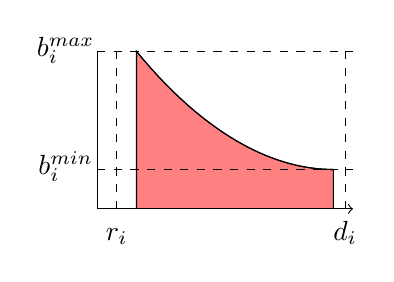
\begin{tikzpicture}
  [scale=0.5]
  \node (O) at (0,0) {};
  \onslide<4->{  
    \path[draw, fill=red!50] (1,0) -- (1,4) parabola [bend at end] (6,1) -- (6,0); 
  }
  \onslide<2->{
    \node[label={[shift={(0,-0.7)}]$r_i$}]  at (0.5,0) {};
    \node[label={[shift={(0,-0.7)}]$d_i$}]  at (6.3,0) {};
    \draw[dashed] (0.5,0) -- (0.5,4);
    \draw[dashed] (6.3,0) -- (6.3,4);
  }
  \onslide<3->{
    \node[label={[shift={(-0.4,-0.4)}]$b_i^{min}$}]  at (0,1) {};
    \node[label={[shift={(-0.4,-0.4)}]$b_i^{max}$}]  at (0,4) {};
    \draw[dashed] (0,1) -- (6.5,1);
    \draw[dashed] (0,4) -- (6.5,4);}
  
  
  \draw (O.center) -- (0,4);
  \draw[->] (O.center) -- (6.5,0);
  
  \draw (1,4) -- (1,0);
  
  
  \path[draw] (1,4) parabola [bend at end] (6,1); 
  
  \draw (6,1) -- (6,0);
\end{tikzpicture}

        \end{column}
      \end{columns}
      \vfill}
    \only<2>{
      \vfill
      \begin{itemize}
      \item Modeled with a continuous resource
      \end{itemize}
      \vfill 
      $\Rightarrow$ \textbf{Continuous Energy-Constrained Scheduling Problem (CECSP) {\scriptsize \color{gray!50!black!50} \it [Artigues \& Lopez, JoS, 2015]}}
      \vfill}
  \end{overlayarea}
\end{frame}

\begin{frame}
  \frametitle{Problem statement}
  \vfill
  Input:\\
  \begin{itemize}
  \item $A=\{1,\hdots,n\}$ a set of non-preemptive tasks
  \item a {\bf continuous}, {\bf cumulative} and {\bf renewable} resource of capacity  $B$
  \end{itemize}
  \vfill
  \onslide<2->{
    Output: A scheduling, i.e. a start time $st_i$, an end time $et_i$ and a resource allocation function $b_i(t)$, such that:
  }
  \begin{overlayarea}{\linewidth}{1cm}
    \only<3>{\[{\color{red!80!black!80}r_i}\le st_i\le et_i \le {\color{red!80!black!80}d_i}\]}
    \only<4>{\[{\color{red!80!black!80}\bmin} \le b_i(t) \le {\color{red!80!black!80}\bmax} \quad \forall t \in \inter[st_i][et_i]\]}
    \only<5>{\[b_i(t)={\color{red!80!black!80}0}\quad \forall t \not\in \inter[st_i][et_i]\]}
    \only<6>{\[\int_{st_i}^{et_i}b_i(t)dt=W_i\]}
    \only<7>{\[\sum_{i\in A}b_i(t) \le {\color{red!80!black!80}B}\]} 
  \end{overlayarea}
  \onslide<2->{
    \begin{center}
      \input{figures/form2_bi.tex}
    \end{center}}
\end{frame}

\begin{frame}
  \frametitle{Example}
  \begin{center}
    \begin{tabular}{cccccc}
      \hline
      $i$ & $r_i$ & $d_i$ & $W_i$ & $b_i^{min}$ & $b_i^{max}$ \\
      \hline
      {\color<2->{red!80!black!80}$1$} &
                                          {\color<2->{red!80!black!80}$0$} & {\color<2->{red!80!black!80}$6$} & {\color<2->{red!80!black!80} $12$} & {\color<2->{red!80!black!80} $1$ }& {\color<2->{red!80!black!80} $5$} \\
      $2$ & $2$ & $6$ & $12$ & $2$ & $5$ \\
      $3$ & $2$ & $5$ & $6$ & $2$ & $2$ \\
      \hline
    \end{tabular}
  \end{center}
  
  \begin{columns}
    \begin{column}{0.45\linewidth}
      \onslide<1->{
        \begin{tikzpicture}
[scale=0.7]
\node (O) at (0,0) {};
\node[label={[shift={(-0.4,0)}]$B=5$}] (B) at (0,5) {};

\onslide<3->{
\node[label={[shift={(-0.4,-0.4)}]\color{red!80!black!80}$b_1^{min}$}] (B) at (0,1) {};
\node[label={[shift={(-0.4,-0.4)}]\color{red!80!black!80}$b_1^{max}$}] (B) at (0,5) {};
}

\node (r1) at (0,-0.5) {{\color<3->{red!80!black!80}$est_1$}}; 
\node (r2) at (2,-0.5) {$est_2$};
\node (r3) at (2,-0.9) {$est_3$};
\node (d1) at (6,-0.5) {{\color<3->{red!80!black!80}$let_1$}};
\node (d2) at (6,-0.9) {$let_2$};
\node (d3) at (5,-0.5) {$let_3$};


\draw[->,>=latex] (6,0) -- (6.5,0);

%\draw (0,0) rectangle (6,5);
\draw[fill=blue!80!black!80] (4,0) -- (6,0) -- (6,5) -- (5,5) -- (5,3) -- (2,3) -- (2,1) --
(4,1) --cycle;
\onslide<2-3>
    {\draw[fill=red!80!black!80] (2,5) -- (2,1) -- (4,1) -- (4,0) -- (0,0) -- (0,5) -- cycle;}
\onslide<3->
    {\draw[fill=red!80!black!80] (2,5) -- (2,1) -- (4,1) -- (4,0) -- (0,0) -- (0,5) -- cycle;}
% \onslide<7>
%     {\draw[fill=red!80!black!80] (2,5) -- (2,0) -- (0,0) -- (0,5)-- cycle;
%       \draw[fill=red!80!black!80,pattern=north west lines, pattern color=red!80!black!80] (2,1) -- (4,1) -- (4,0)-- (2,0) -- cycle;
%     }
% \onslide<8->
%     {\draw[fill=red!80!black!80,pattern=north west lines, pattern color=red!80!black!80] (2,1) -- (4,1) -- (4,0)-- (0,0) --(0,5)--(2,5) -- cycle;
%     }
\draw[fill=orange!80!black!80]  (2,3) -- (5,3) -- (5,5) -- (2,5) --cycle;


\node (2) at (4,2) {\LARGE $2$};
\node (1) at (1,2) {\LARGE $1$};
\node (3) at (3.5,4) {\LARGE $3$};
\foreach \i in {0,...,5}
{
  \draw (\i,-0.3) -- (\i,0);
  \draw (-0.3,\i) -- (0,\i);
}

 \draw (6,-0.3) -- (6,0);

\end{tikzpicture}

      }
    \end{column}
    \hfill
    \begin{column}{0.45\linewidth}
      \newbox\hautbox \setbox\hautbox=\hbox{\vphantom{\rule[-0.4cm]{0cm}{0.9cm}}}
      \begin{tabular}{@{\usebox{\hautbox}}l}
        \onslide<3->{$\int_0^{4} b_1(t)dt=?$} \\
        \onslide<4->{$\int_0^{2}${\color<4>{red!80!black!80}{$5$}}$dt +\int_2^{4}${\color<4>{red!80!black!80}{$1$}}$dt$\\
        $=10+2=12$}
      \end{tabular}
    \end{column}
    \hfill
  \end{columns}
\end{frame}


\begin{frame}{The CECSP : limitations}
  \vfill
  \begin{itemize}
  \item Consider that the resource consumed by the task is proportional to
    the energy received by the task.
    \vfill
    \pause
  \item Not always the case...
  \end{itemize}
  \vfill
  \pause
  \begin{block}{Example of the foundry}
    Give twice more power to the furnace $\not\Rightarrow$ Task
    finishes twice faster... 
  \end{block}
  \vfill

\end{frame}

  % \begin{block}{Example in parallel architecture}
  %   \begin{itemize}
  %   \item a set of tasks has to be scheduled on parallel processors;
  %     \pause
  %   \item resource : processors;
  %     \pause
  %   \item energy : elementary operation;
  %     \pause
  %   \item Typical power speed function:  $b^{\alpha} , \ 0 <
  %     \alpha \le 1$ (may be different for each task)
  %     \pause
  %   \end{itemize}
  % \end{block}


\begin{frame}{The CECSP : limitations}
  \begin{itemize}
  \item   $\Rightarrow$ We need to model {\bf conversion functions} $f_i$.
    \vfill
    \pause
  \item  We have considered the case where $f_i(b)$ is non-decreasing,
    continuous and  
    \pause
    \begin{enumerate}
      \vspace{0.5cm}
    \item linear: $f_i(b)=a_i*b+c_i(1-\delta_{b0})$ 

      \vspace{0.1cm}
      $\rightarrow$ the {\bf CECSP$_{lin}$}
      \vspace{0.5cm}
      \pause
    \item concave and piecewise linear: if $f$ has $P$ pieces,
      $f_i(b)=a_{ip}*b+c_{ip}(1-\delta_{b0}) , p \in \{1,\dots,P\}$

      \vspace{0.1cm}
      $\rightarrow$ {\bf the CECSP$_{cpwl}$} 
    \end{enumerate}
    \vfill
    \pause
  \item   \[W_i=\int_{st_i}^{et_i}b_i(t)dt \rightarrow
      W_i=\int_{st_i}^{et_i}{\color{red!80!black!80}\mathbf{f_i}(}b_i(t)
      {\color{red!80!black!80})}dt\]   
    \vfill
    \pause
  \item   linear and concave piecewise linear approximation of more
    general efficiency functions.
  \end{itemize}
  \vfill
\end{frame}

\begin{frame}
  \frametitle{Concave Efficiency Function}
  $f_i$ are continuous, non-decreasing and {\bf concave} efficiency functions 
  \vfill
  \begin{columns}
    \begin{column}{0.45\linewidth}
      \begin{figure}
        \centering
        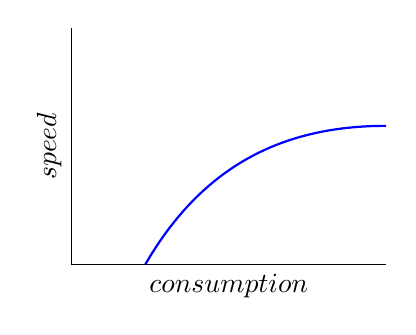
\begin{tikzpicture}
          \node (O) at (0,0) {};
          \draw (0,0) -- (4,0) node[midway,below] {$consumption$};
          \draw (0,0) -- (0,3) node[midway,left] {\rotatebox{90}{$speed$}};
          \draw[thick,blue] (0.94,0) to [bend left] (4,1.76);
        \end{tikzpicture}
        \caption{Speed vs. fuel consumption\footnotemark}
      \end{figure}
    \end{column}
    \hfill
    \begin{column}{0.45\linewidth}      
      \vspace{0.2cm}
      \begin{figure}
        \centering    
        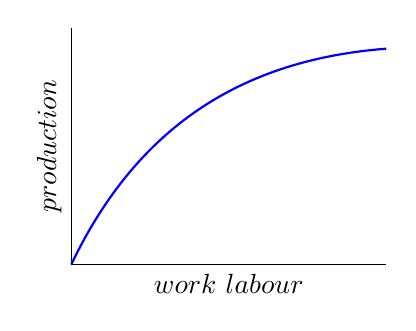
\begin{tikzpicture}
          \node (O) at (0,0) {};
          \draw (0,0) -- (4,0) node[midway,below] {$work\ labour$};
          \draw (0,0) -- (0,3) node[midway,left] {\rotatebox{90}{$production$}};
          \draw[thick,blue] (0,0) to [bend left] (4,2.74);
        \end{tikzpicture}      
        \caption[\footnotesize]{ Work Labour vs. production rate\footnotemark}
      \end{figure}
    \end{column}
    \hfill
  \end{columns}
  \footnotetext[1]{\tiny Algebra Symposium: Optimizing Fuel Consumption}
  \footnotetext[2]{\tiny Non-convex agreggative technology
    and optimal economic growth}
\end{frame}


\begin{frame}{Approximation by below of efficiency functions}
  \vfill
  \begin{columns}
    \begin{column}{0.5\linewidth}
      \begin{figure}[!htb]
\captionsetup{justification=centering}
        \centering
        \begin{tikzpicture}
          [xscale=0.55,yscale=0.35]
          \node (O) at (0,0) {};
          
          \draw[dotted] (7,0) node[below] {$\bmax$} -- (7,7);
          \draw[dotted] (1,0) node[below] {$\bmin$} -- (1,7);
          \draw[->] (O.center) -- (8,0) node [below] {$b$};
          \draw[->] (O.center) -- (0,7) node [left] {$f(b)$};
          \draw[gray!80] (0,0.01) parabola bend (0.5,0.01) (3.6,3.4);
          \draw[gray!80] (3.6,3.4) parabola bend (6.5,6) (7.5,6);

          \draw[densely dashed] (1.25,0) -- (7,6);
        \end{tikzpicture}
        \caption{Approximation by a linear function}
      \end{figure}
    \end{column}
    \pause
    \begin{column}{0.5\linewidth}
      \begin{figure}[!htb]
        \centering
\captionsetup{justification=centering}
        \begin{tikzpicture}
          [xscale=0.55,yscale=0.35]
          \node (O) at (0,0) {};
          
          \draw[dotted] (7,0) node[below] {$\bmax$} -- (7,7);
          \draw[dotted] (1,0) node[below] {$\bmin$} -- (1,7);
          \draw[->] (O.center) -- (8,0) node [below] {$b$};
          \draw[->] (O.center) -- (0,7) node [left] {$f(b)$};
          \draw[gray!80] (0,0.01) parabola bend (0.5,0.01) (3.6,3.4);
          \draw[gray!80] (3.6,3.4) parabola bend (6.5,6) (7.5,6);

          \draw[densely dashed]  (6,5.9) -- (7,6);
          \draw[densely dashed]  (6,5.9) -- (5,5.3);
          \draw[densely dashed] (4,4.05) -- (5,5.3);
          \draw[densely dashed]  (3,2.1) -- (4,4.05);
          \draw[densely dashed] (1.5,0) -- (3,2.1);
        \end{tikzpicture}
        \caption{Approximation by a concave piecewise linear function}
      \end{figure}
    \end{column}
  \end{columns}

\end{frame}

\begin{frame}{Example for the CECSP$_{lin}$}
  

\begin{columns}
  \begin{column}{0.5\linewidth}
    \begin{center}
      {\small \begin{tabular}{|M{0.4cm}|M{0.4cm}M{0.4cm}M{0.4cm}M{0.4cm}M{0.4cm}M{1.2cm}|}
        \hline
        $i$ & $r_i$ & $d_i$ & $W_i$ & $\bmin$ & $\bmax$ & $f_i(b)$\\[1mm]
        \hline
        1 & 0 & 2 & 6 & 3 & 3 & $b$\\[1mm]
        \color<3->{red!80!black!80}2 & \color<3->{red!80!black!80}1 & \color<3->{red!80!black!80}5 & \color<3->{red!80!black!80}22 & \color<3->{red!80!black!80}3 & \color<3->{red!80!black!80}4 & \color<3->{red!80!black!80}$\rightarrow$ \\[1mm]
         3 & 0 &6 & 45 & 1 & 5 & $3b+1$\\[1mm]
        \hline
        \multicolumn{7}{c}{}
      \end{tabular}}
    \end{center}
  \end{column}
\hfill
    \begin{column}{0.4\linewidth}
\begin{tikzpicture}
[xscale=0.8,yscale=0.45]
\node (O) at (2,5) {};
\draw[->] (2,4) -- (5.5,4) node[below] {$b$}; 
\draw[dashed] (2,4) -- (2,5.5);
\draw[->] (2,5.5) -- (2,10) node[left] {$f_2(b)$};


\path[draw] (3,6) -- (4,8) -- (5,9) ;

\draw[dotted] (3,4) node[below] {\footnotesize $3$} -- (3,10);
\draw[dotted,color=gray!70] (4,4) node[below,color=black] {\footnotesize $4$}
-- (4,10);
\draw[dotted] (5,4) node[below] {\footnotesize $5$} -- (5,10);

\draw (2,6) node[left] {\footnotesize $6$};
\draw (2,8) node[left] {\footnotesize $8$};
\draw (2,9) node[left] {\footnotesize $9$};
\end{tikzpicture}
\end{column}
\end{columns}
\pause
  \begin{columns}
    \begin{column}{0.45\linewidth}
      \onslide<2->{
        \centering
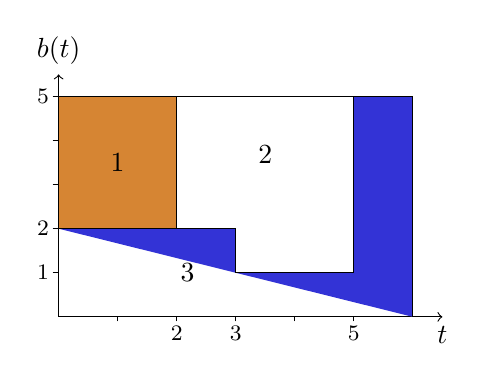
\begin{tikzpicture}
[xscale=0.75,yscale=0.56]
\node (O) at (0,0) {};
\draw[->] (0,0) -- (6.5,0) node[below] {$t$};
\draw[->] (0,0) -- (0,5.5) node[above] {$b(t)$};

\draw[fill=orange!80!black!80] (0,2) rectangle (2,5) node[midway] {$1$};
\path[draw,fill=blue!80!black!80] (0,2) -- (3,2) -- (3,1) node[left=0.4cm] {$3$} -- (5,1) -- (5,5) -- (6,5)  -- (6,0);
\draw[fill=red!80!black!80] (2,5) -- (5,5) node[midway,below=0.5cm] {$2$};

\draw (0,1) node[left] {\footnotesize $1$};
\draw (0,2) node[left] {\footnotesize $2$};
\draw (0,5) node[left] {\footnotesize $5$};


\draw (2,0) node[below] {\footnotesize $2$};
\draw (3,0) node[below] {\footnotesize $3$};
\draw (5,0) node[below] {\footnotesize $5$};

\foreach \i in {1,...,5}{
\draw (\i,-0.1) -- (\i,0);
\draw (-0.1,\i) -- (0,\i);
}
\end{tikzpicture}

      }
    \end{column}
    \hfill
       \begin{column}{0.45\linewidth}{
\vspace{-0.1cm}       
       \small
      \newbox\hautbox \setbox\hautbox\hbox{\vphantom{\rule[-0.4cm]{0cm}{0.8cm}}}
      \begin{tabular}{@{\usebox{\hautbox}}l}
        \onslide<4->{$\int_2^{5} f_2(b_2(t))dt=?$} \\
        \onslide<5->{$\int_2^{3} f_2(3) dt$}\onslide<6->{$+\int_3^{5} f_2(4) dt$=}\\
	    \onslide<7->{$\int_2^{3} 6 dt$}\onslide<8->{$+\int_3^{5} 8 dt$=}\\
       \onslide<9->{$6$}\onslide<10->{$+16=$}\onslide<11->{$22$}\onslide<12->{$\
        \neq
        \int_2^5 b_2(t)dt = 11 $}\\
              \end{tabular}}
    \end{column}
    \hfill
  \end{columns}

\end{frame}


\begin{frame}
  \frametitle{Problem statement}
  \vfill
 {\small  {\bf Input: } 
  \begin{itemize}
  \item $A=\{1,\hdots,n\}$ a set of non-preemptive tasks
  \item a continuous, cumulative and renewable resource of capacity  $B$
  \end{itemize}
  \vspace{0.5cm}
  {\bf Output:} a start/end time $st_i/et_i$ and a res. allocation function
  $b_i(t)$ s.t.:
  {\footnotesize
    \begin{align}
    r_i\le st_i\le
   et_i \le d_i & & \tag{{\it \scriptsize
                                                     time-window}}\\
    \bmin \le b_i(t) \le \bmax & & \forall t
                                                                 \in \inter[st_i][et_i] \tag{{\it \scriptsize min/max consump.}}\\
    b_i(t)=0 & &
                                               \forall t \not\in \inter[st_i][et_i] \tag{{\it \scriptsize no
                                               consump.}}\\ 
    \int_{st_i}^{et_i}f_i(b_i(t))dt=W_i
                                                 & &\tag{{\it \scriptsize energy}} \\
    \sum_{i\in A}b_i(t) \le B & & \tag{{\it
                                                                \scriptsize cumulative}}
  \end{align}
}

  \vspace{0.5cm}
{\bf Possible objective:} $\qquad $ minimize  $\sum_{i\in A}
\int_{st_i}^{et_i} b_i(t)dt $}
\end{frame}

\begin{frame}
  \frametitle{Solution methods}
  \vfill
  \begin{description}[Properties]
  \item[Properties] {\small
      \begin{itemize}
      \item study of the structural properties of the problem:
        {\footnotesize Dominance rules, complexity analysis, polynomial cases...}
      \end{itemize}}
    \vfill
    \pause
  \item[CP] {\small
      \begin{itemize}
      \item satisfiability test (checker): {\footnotesize Energetic
          reasoning, Flow based checker...}
      \item filtering algorithm: {\footnotesize Energetic reasoning, time-table
          disjunctive reasoning...}
      \item discrete model
      \end{itemize}}
    \vfill
    \pause
  \item[MILP] {\small
      \begin{itemize}
      \item MILP model: {\footnotesize time-indexed, event-based...}
      \item valid inequalities
      \item polyhedral results
      \end{itemize}}
    \vfill
    \pause
  \item[Hybrid] {\small
      \begin{itemize}
      \item ``CP-like branching'' + MILP 
      \item valid inequalities deduced from ER
      \end{itemize}}
  \end{description}
\end{frame}
